\item[(a)]
\section*{Task (a)}

\subsection*{Problem Statement}
Consider the analog signal
\[ x(t) = 1 + 0.5 \cos \left(2 \pi f_{1} t \right) + 2 \sin \left(2 \pi f_{2} t \right) + \sin \left(2 \pi f_{3} t \right) \]
with \( f_{1} = 2 \, \text{kHz} \), \( f_{2} = 4 \, \text{kHz} \), and \( f_{3} = 6 \, \text{kHz} \).

a) Sketch the Fourier transform of \( x(t) \) and plot the analog signal \( x(t) \) in Python using a time vector \( t = 0:1 \times 10^{-6}:1 \times 10^{-3} \).

\subsection*{Theoretical Background}
The Fourier transform is a mathematical operation that transforms a time-domain signal into its frequency-domain representation. It is crucial for analyzing the frequency components of signals.

Given an analog signal \( x(t) \), its continuous Fourier transform \( X(f) \) is defined as:
\[ X(f) = \int_{-\infty}^{\infty} x(t) e^{-j 2 \pi f t} \, dt \]

For a signal consisting of sinusoids, the Fourier transform will show spikes at the corresponding frequencies.

\subsection*{Mathematical Derivation}
The given signal is:
\[ x(t) = 1 + 0.5 \cos \left(2 \pi f_{1} t \right) + 2 \sin \left(2 \pi f_{2} t \right) + \sin \left(2 \pi f_{3} t \right) \]

The Fourier transform of this signal consists of delta functions at the frequencies of the cosine and sine terms:
\[ X(f) = \delta(f) + 0.25 \left[ \delta(f - f_1) + \delta(f + f_1) \right] - j \left[ \delta(f - f_2) - \delta(f + f_2) \right] - 0.5 j \left[ \delta(f - f_3) - \delta(f + f_3) \right] \]

where:
- The delta function \( \delta(f) \) represents the constant term.
- The cosine term \( 0.5 \cos(2 \pi f_{1} t) \) contributes to delta functions at \( \pm f_1 \).
- The sine terms contribute to delta functions at \( \pm f_2 \) and \( \pm f_3 \), with imaginary coefficients indicating phase shifts.

\subsection*{Python Implementation and Plot}
The plot Figure~\ref{fig:ex1_a_plot} below illustrates the time-domain signal, and Figure~\ref{fig:ex1_a_fft} shows its Fourier transform:

\begin{figure}[h]
    \centering
    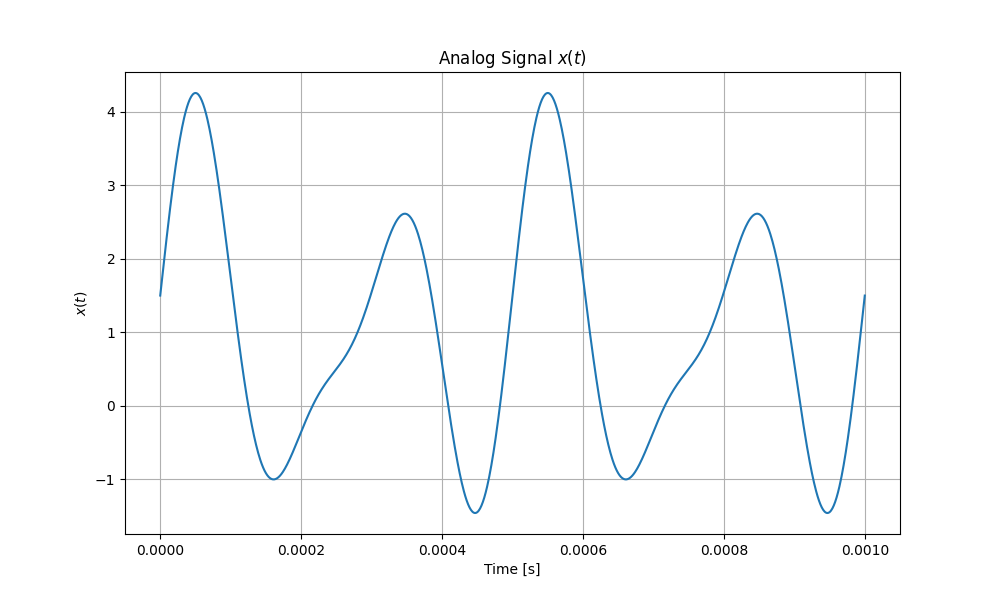
\includegraphics[width=0.8\textwidth]{fig/ex1_a_plot.png}
    \caption{Analog Signal $x(t)$}
    \label{fig:ex1_a_plot}
\end{figure}

\begin{figure}[h]
    \centering
    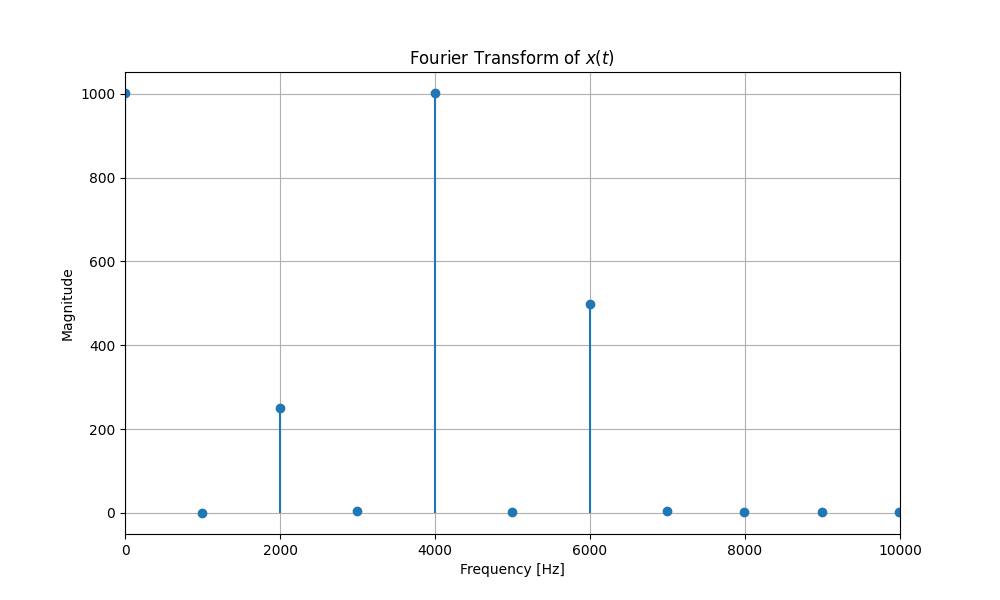
\includegraphics[width=0.8\textwidth]{fig/ex1_a_fft_stem.png}
    \caption{Fourier Transform of $x(t)$}
    \label{fig:ex1_a_fft}
\end{figure}

\subsection*{Conclusion}
The Fourier transform of the given signal shows spikes at the frequencies \( f_1 = 2 \, \text{kHz} \), \( f_2 = 4 \, \text{kHz} \), and \( f_3 = 6 \, \text{kHz} \), corresponding to the cosine and sine terms in the signal. The plot of the analog signal \( x(t) \) illustrates its time-domain behavior over the interval from 0 to 1 ms, and the Fourier transform plot shows the frequency-domain representation with spikes at the expected frequencies.
